\section{Comparativas}

A continuación se exponen los gráficos generados a partir de los resultados de los experimentos que ideamos e implementamos con el fin de hacer un análisis empirico del costo temporal y la calidad de los resultados obtenidos a partir del algoritmo goloso (Ejercicio 3) y de la vecindad 1 del algoritmo de búsqueda local (Ejercicio 4). 

Para ello, separamos este apartado en la observación de tres conjuntos de resultados:

\begin{itemize}
\item {Los obtenidos a partir de grafos completos}
\item {Los obtenidos a partir de grafos cíclicos}
\item {Los obtenidos a parir de grafos bipartitos completos}
\end{itemize}

Consideramos que hacerlo fue de especial relevancia, dado que al incrementar individualmente el valor de parámetros independientes es factible que se terminen realizando experimentos sobre grafos estructuralmente distintos, con poca o ninguna relación en cuanto a sus propiedades.\\
Los resultadoss se observan a continuación:\\


\subsection {Resultados obtenidos a partir de grafos cíclicos} 

 \begin{figure}[H]
    \begin{center}
  	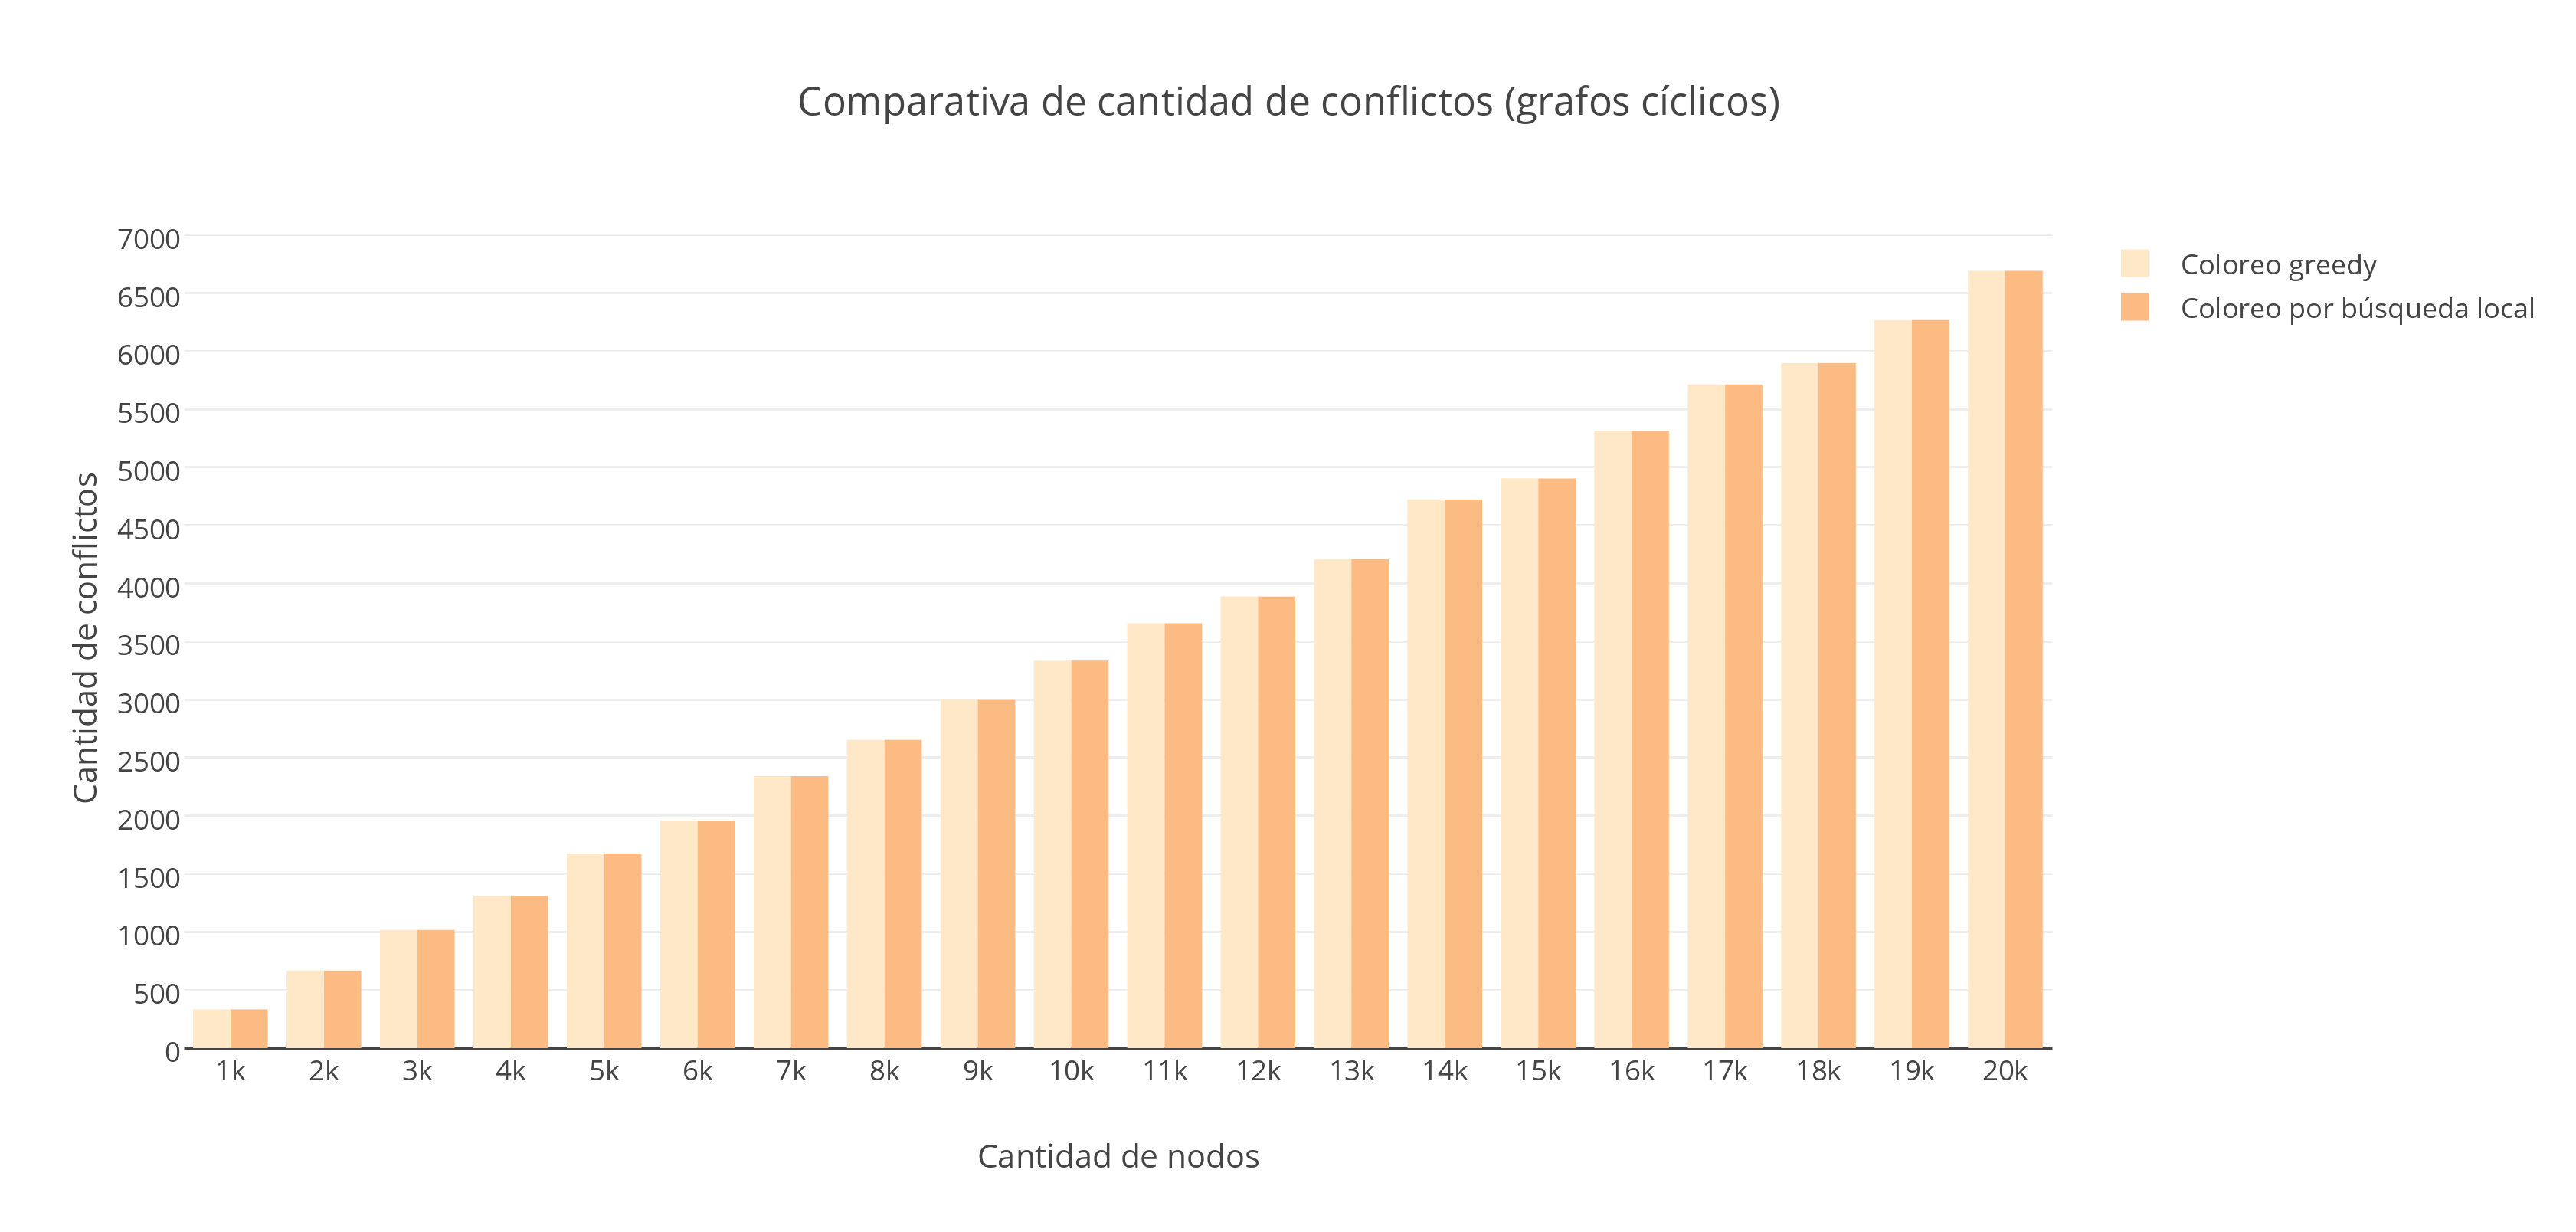
\includegraphics[width=18cm]{imagenes/Ej5/ComparacionConflictosCiclico.png}
 	\label{ComparacionConflictosCiclico}
    \end{center}
  \end{figure}

 \begin{figure}[H]
    \begin{center}
  	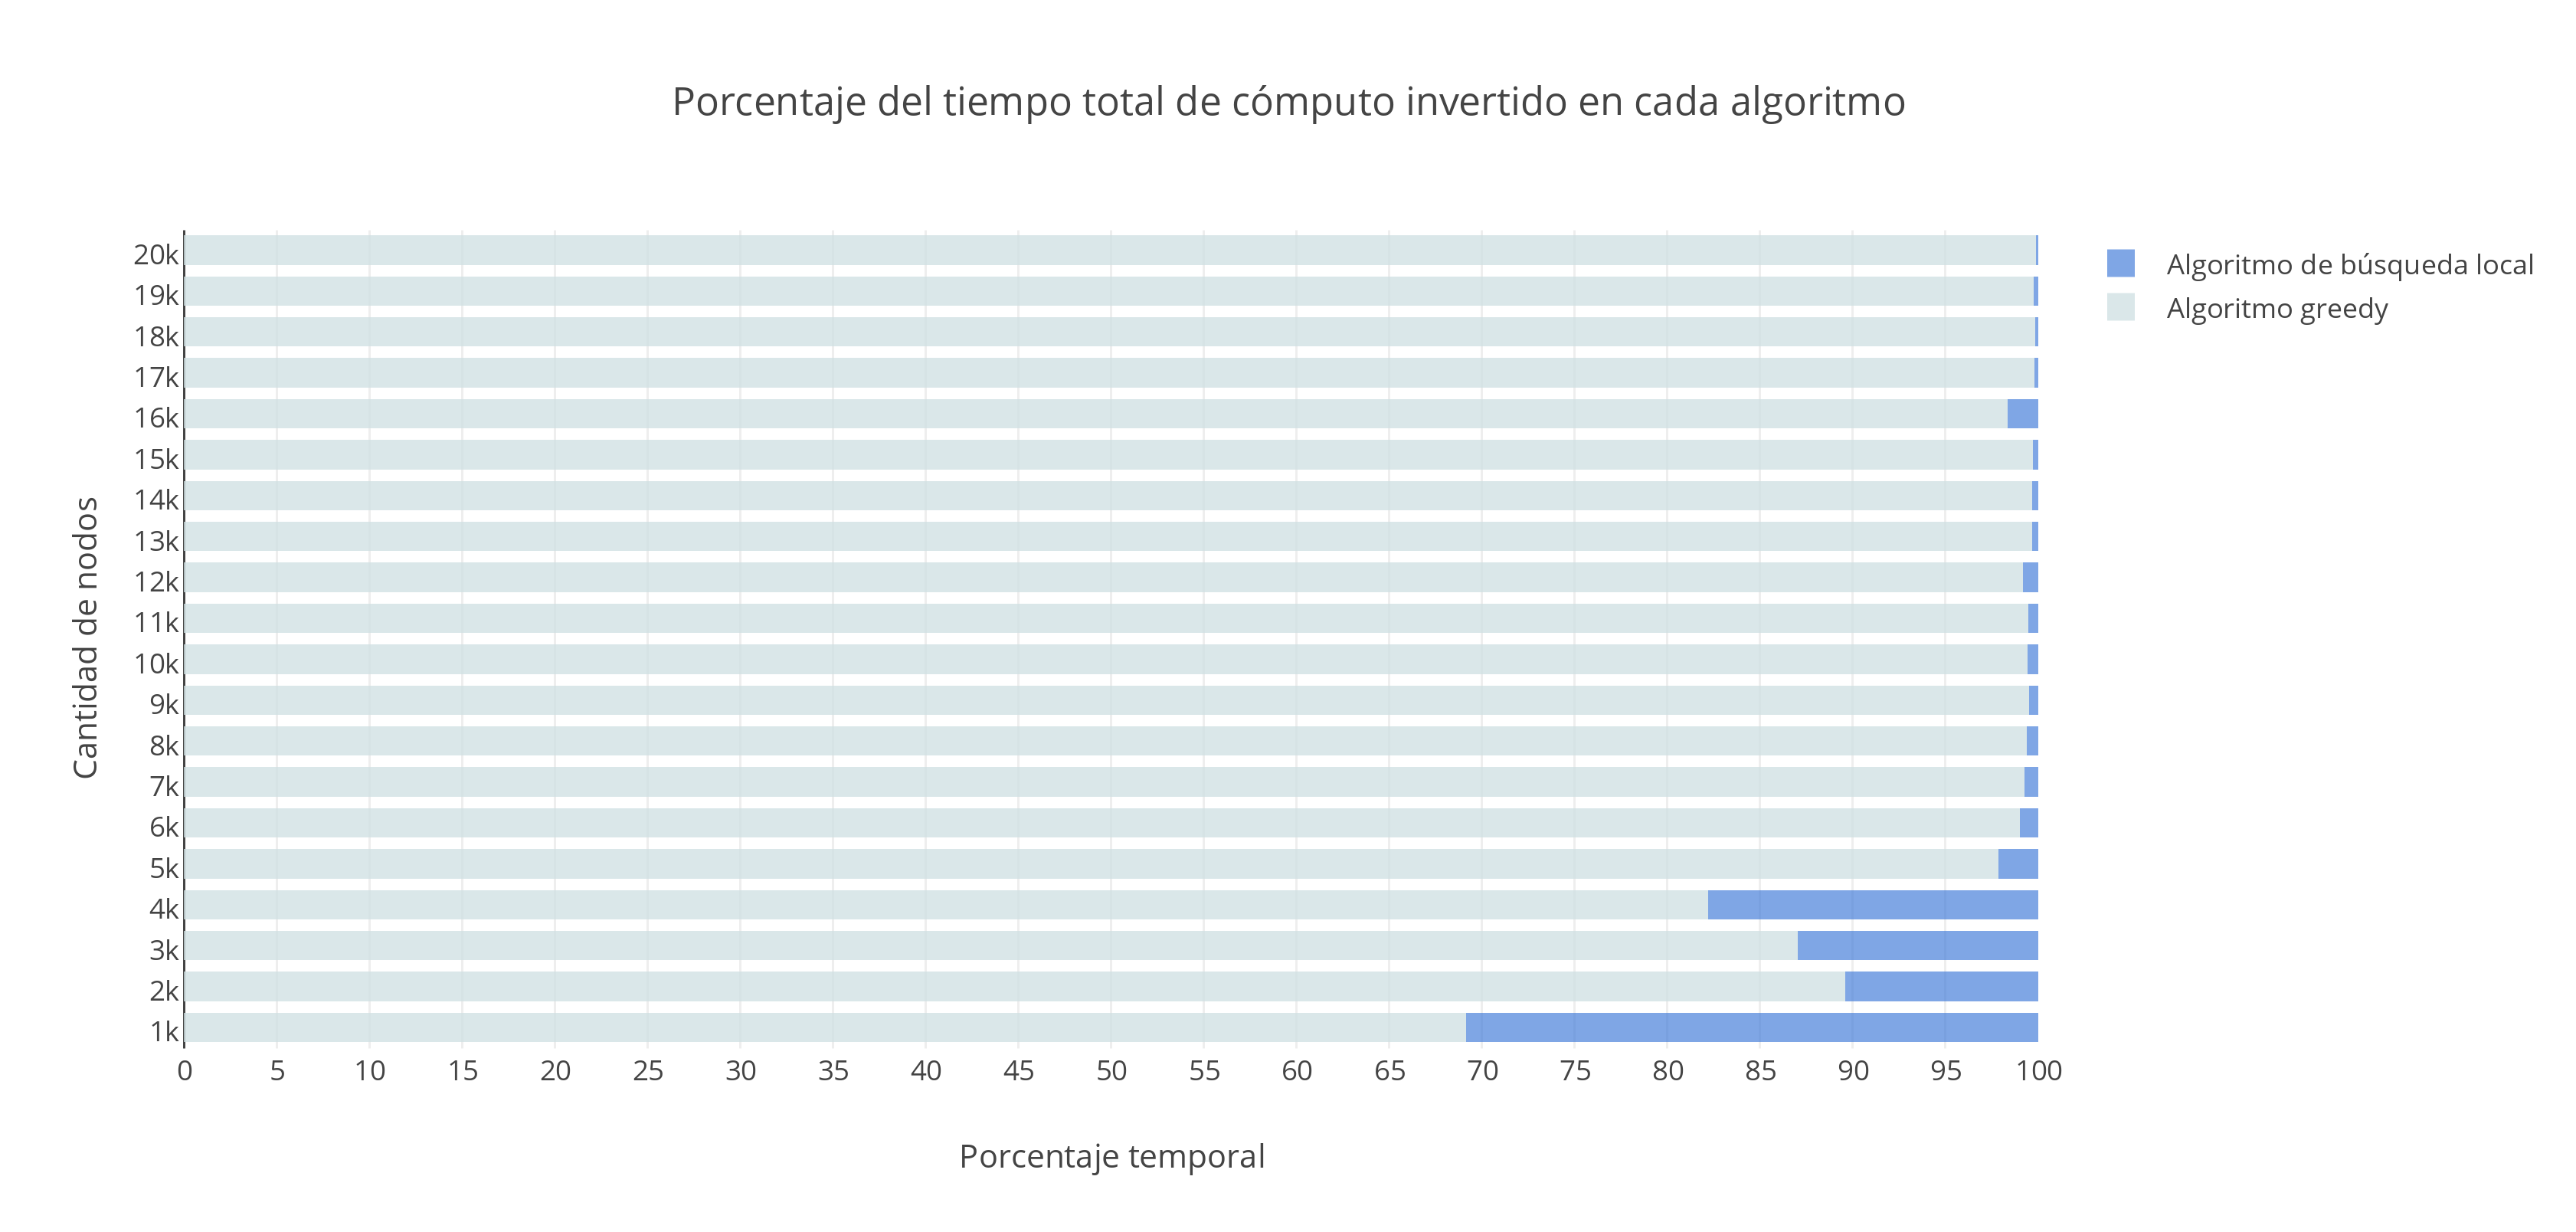
\includegraphics[width=18cm]{imagenes/Ej5/ComparacionTiemposCiclico.png}
 	\label{ComparacionTiemposCiclico}
    \end{center}
  \end{figure}

 \begin{figure}[H]
    \begin{center}
  	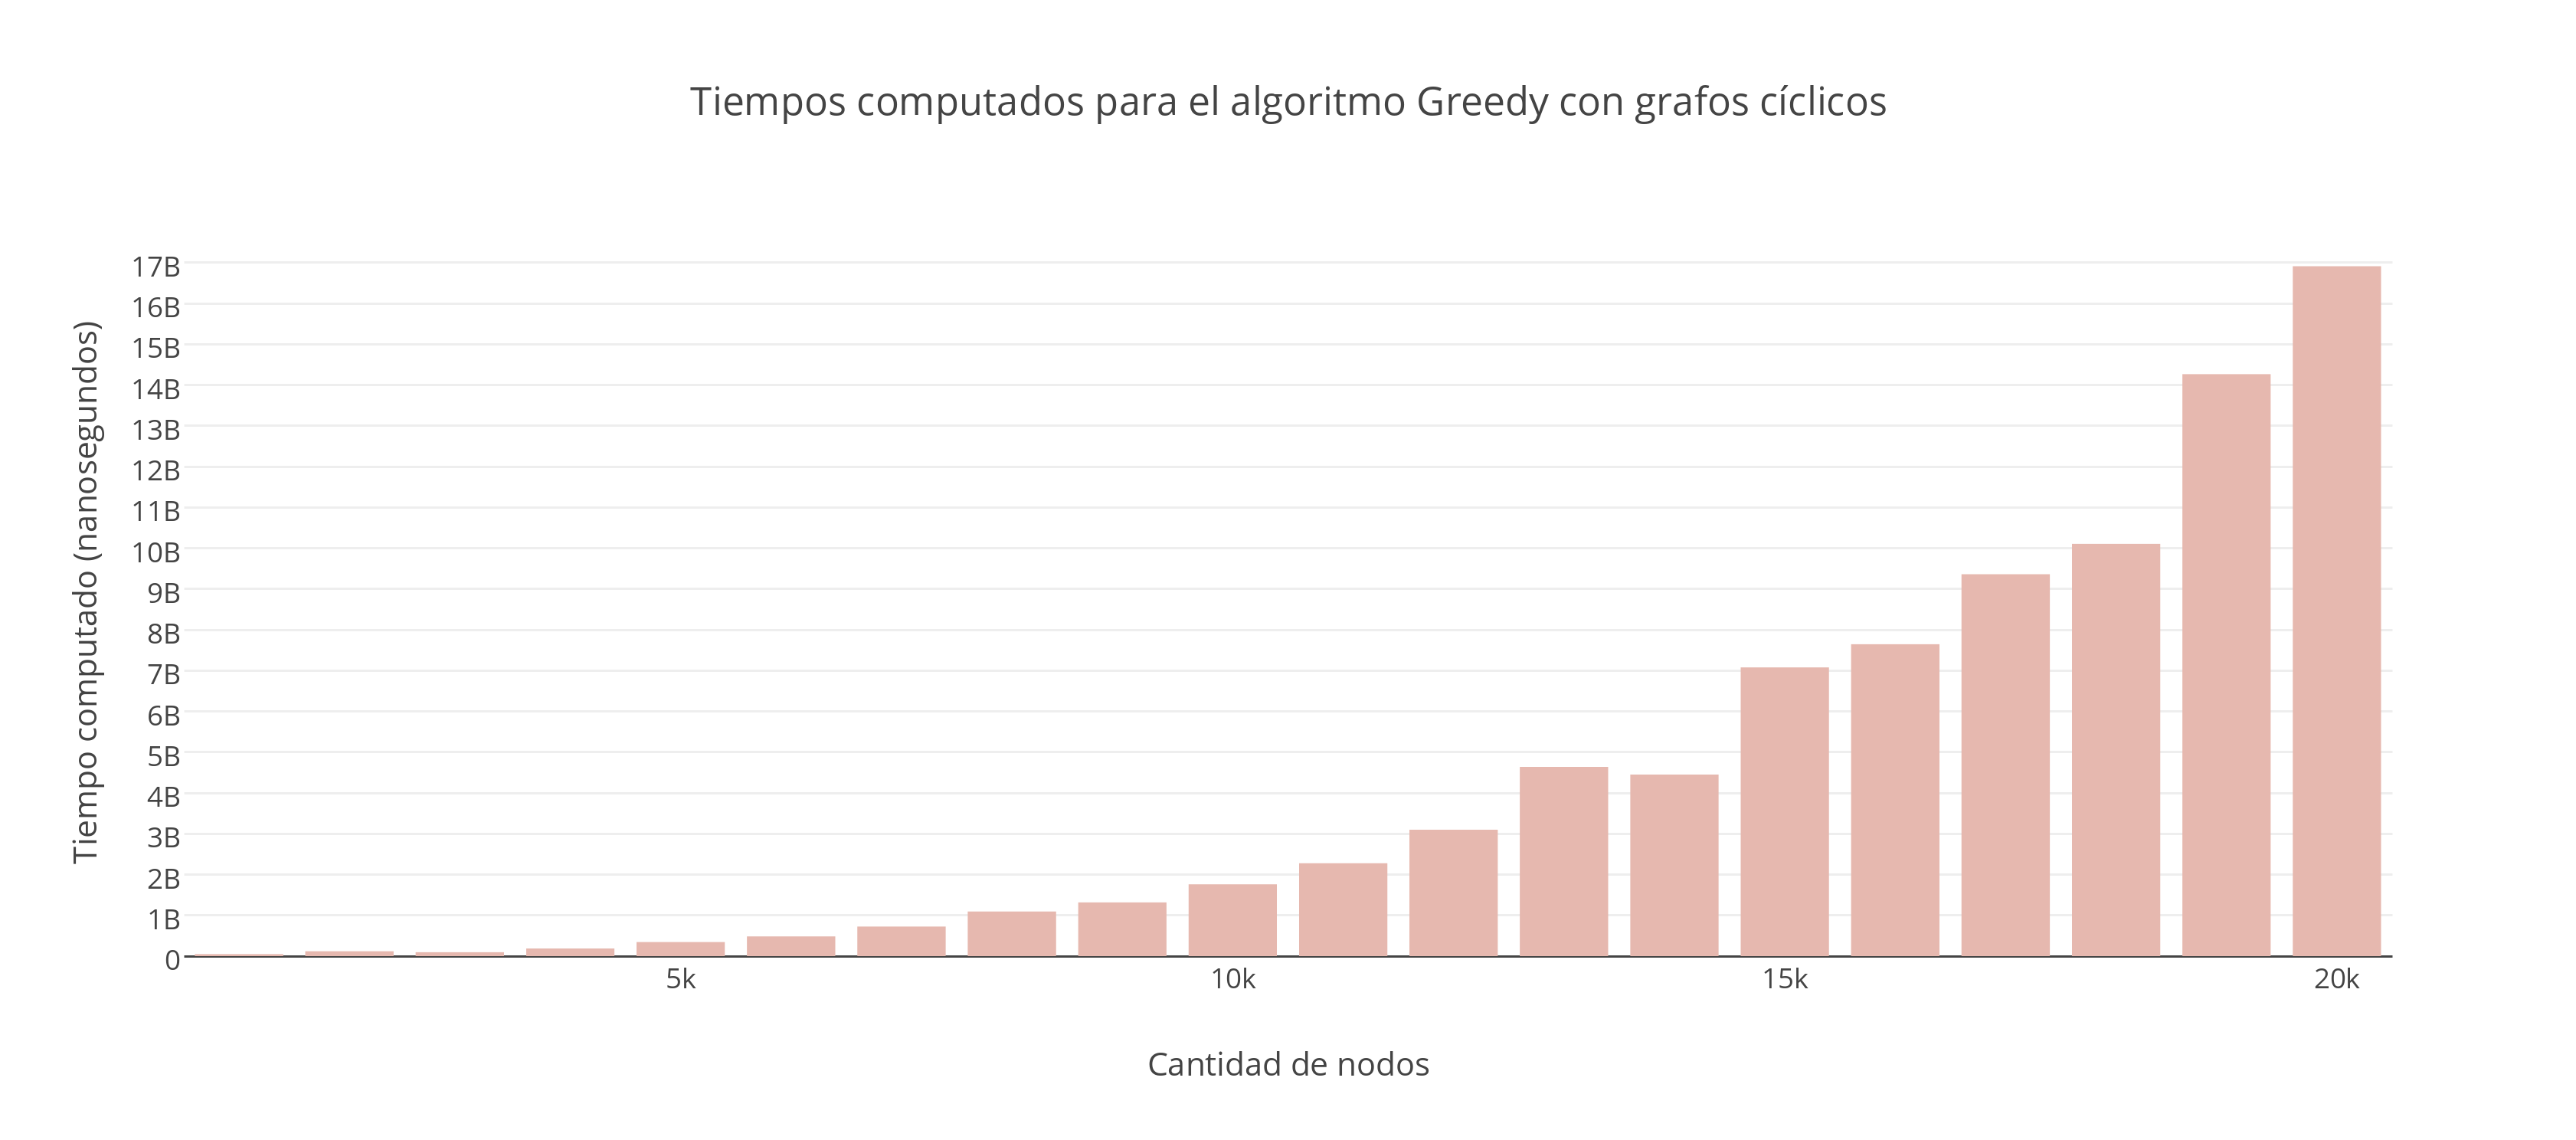
\includegraphics[width=18cm]{imagenes/Ej5/TiempoGreedyCiclico.png}
 	\label{TiempoGreedyCiclico}
    \end{center}
  \end{figure}

 \begin{figure}[H]
    \begin{center}
  	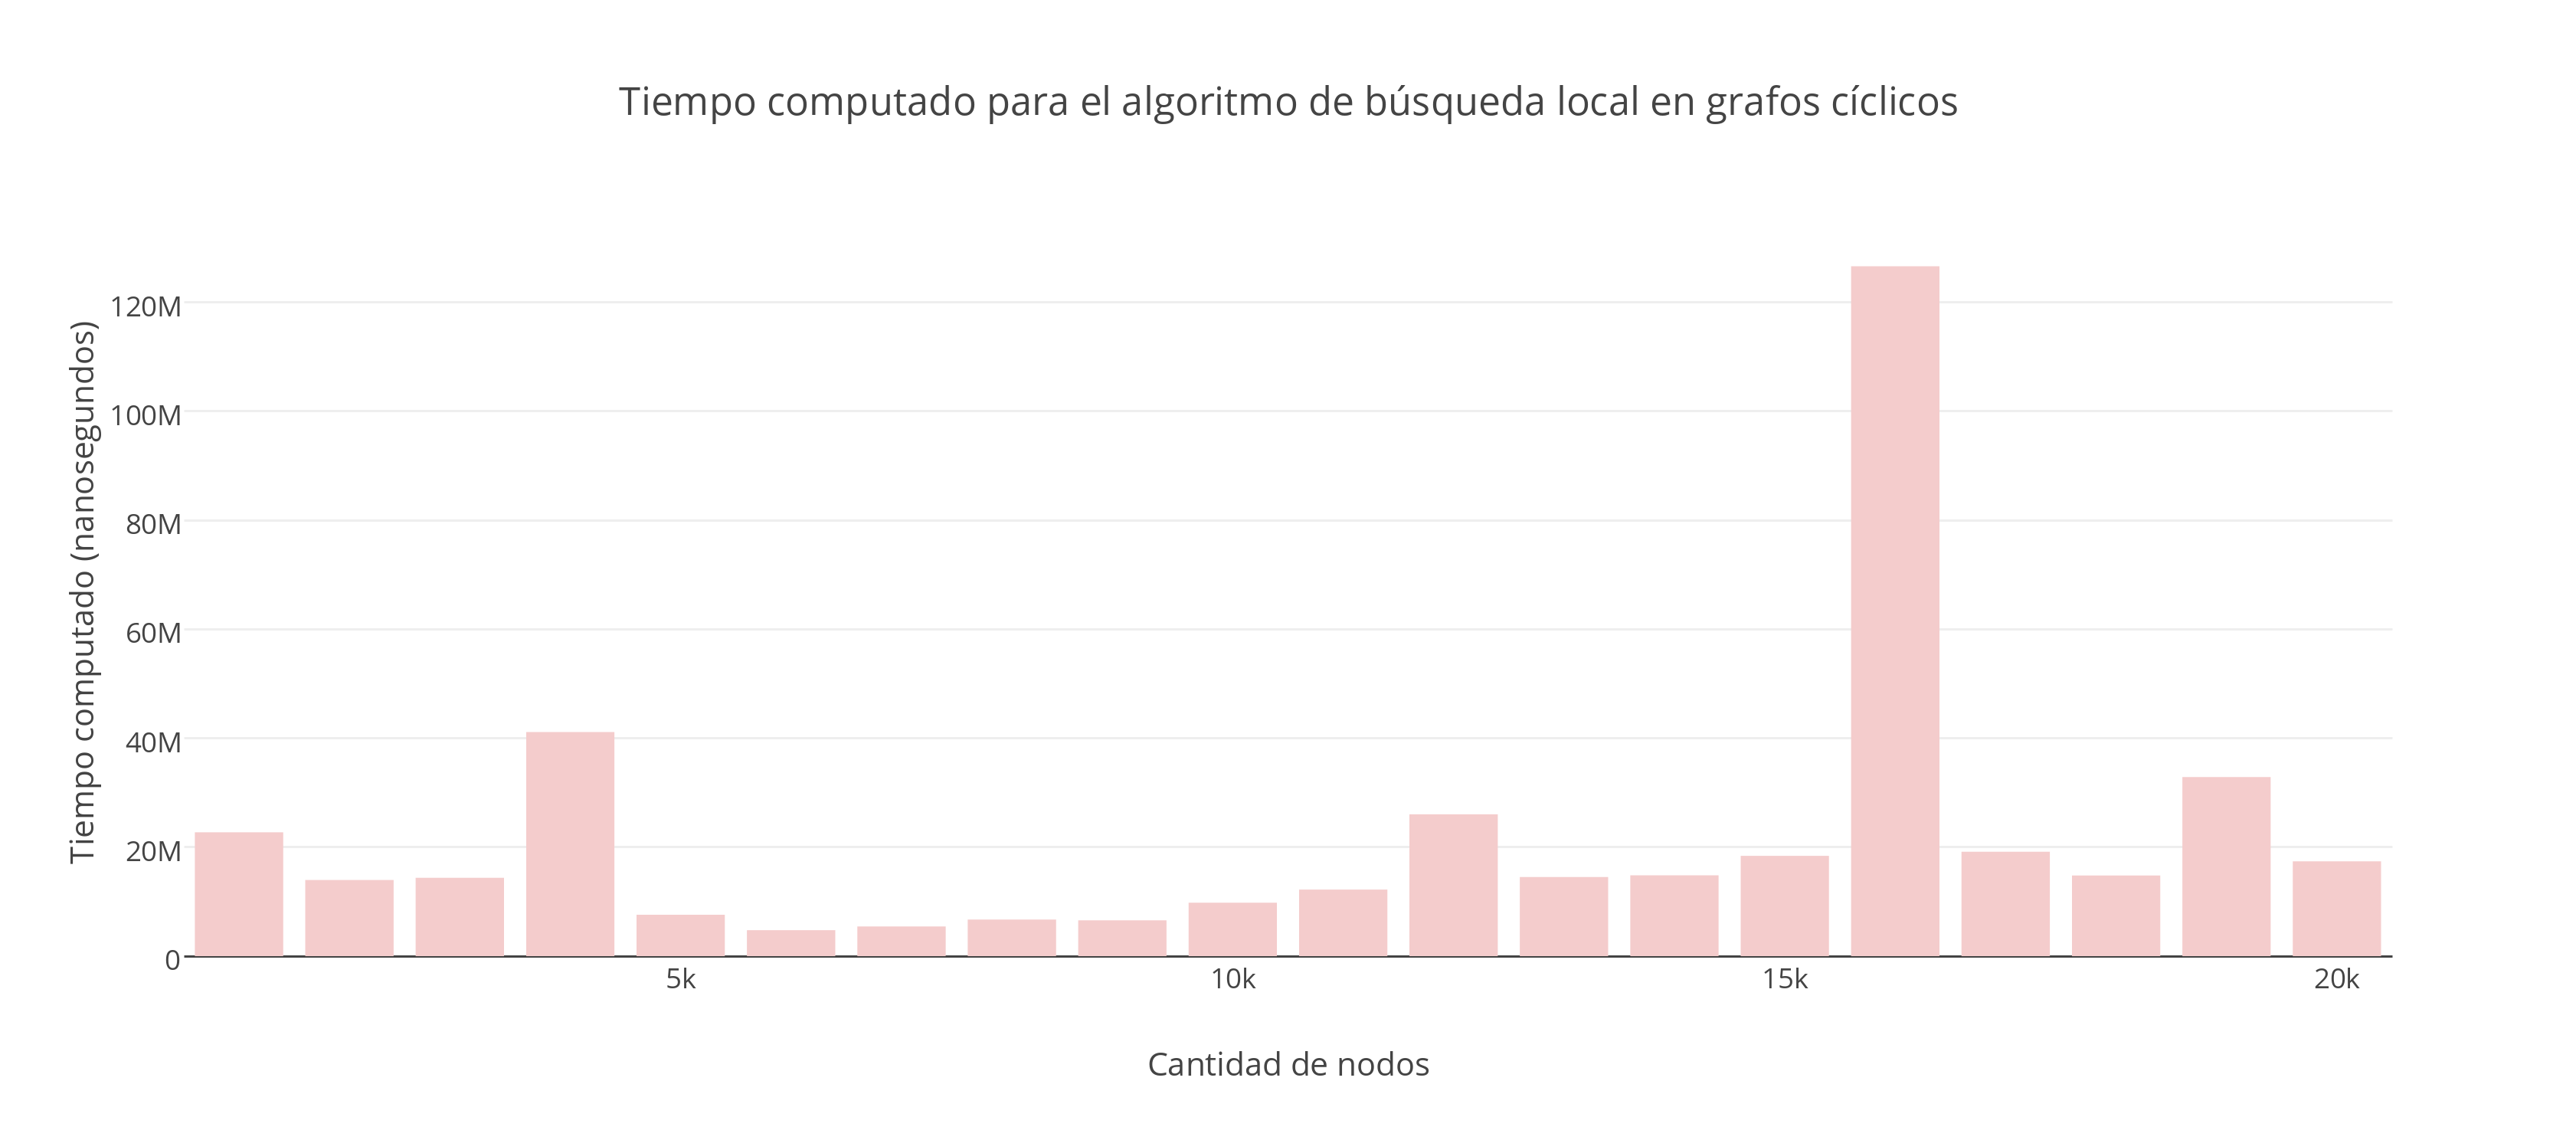
\includegraphics[width=18cm]{imagenes/Ej5/TiempoLocalCiclico.png}
 	\label{TiempoLocalCiclico}
    \end{center}
  \end{figure}

\subsection {Resultados obtenidos a partir de grafos completos} 


 \begin{figure}[H]
    \begin{center}
  	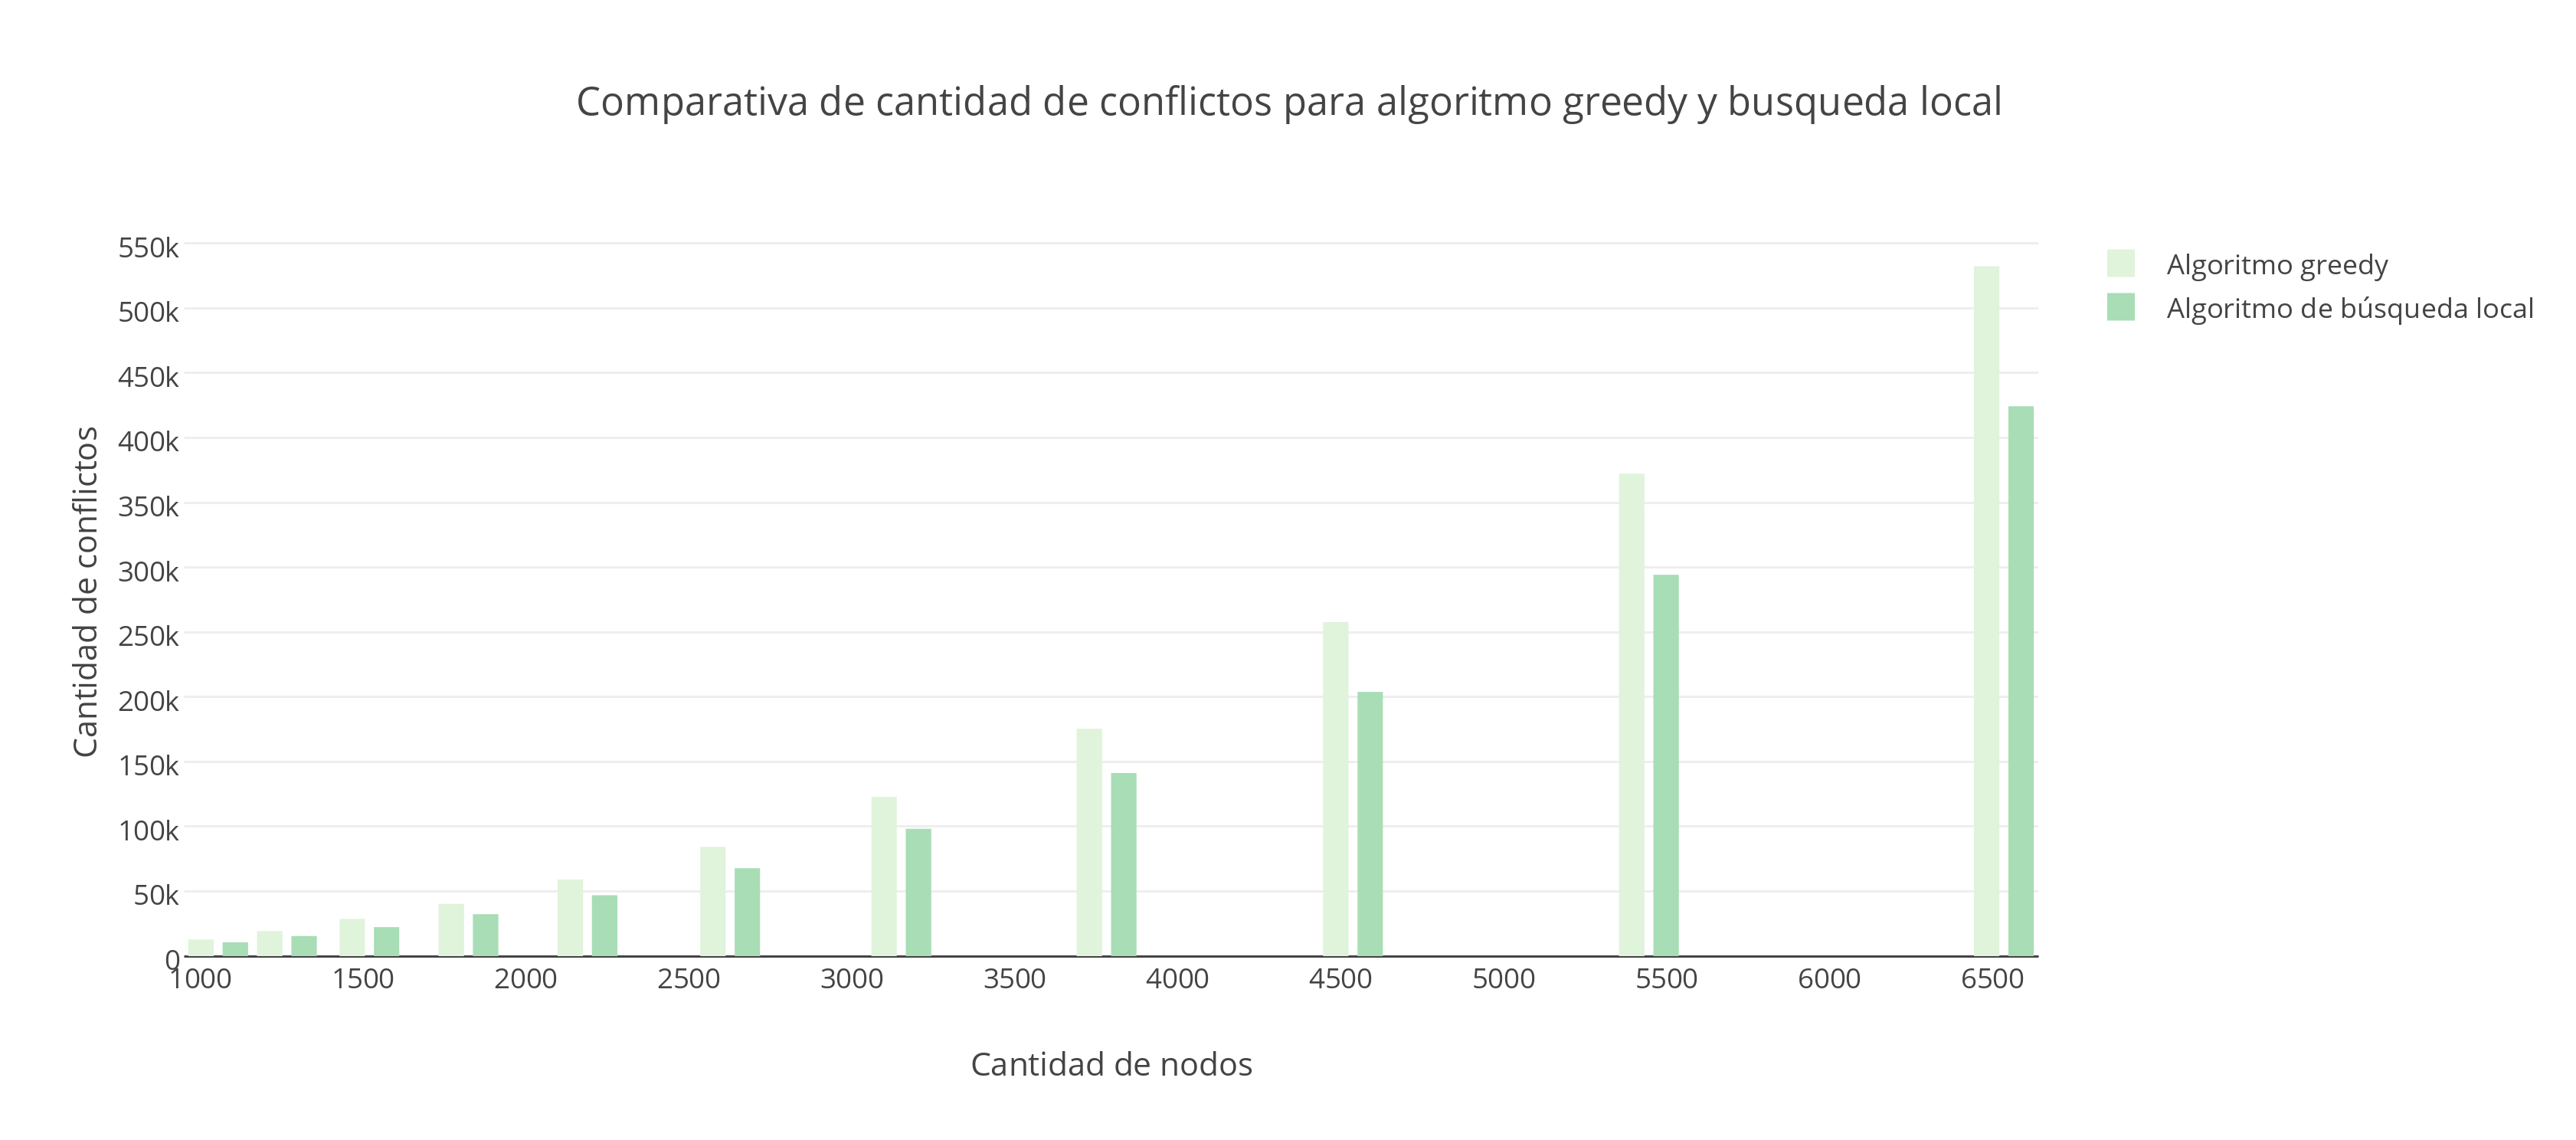
\includegraphics[width=18cm]{imagenes/Ej5/ComparacionConflictosCompleto.png}
 	\label{ComparacionConflictosCompleto}
    \end{center}
  \end{figure}

 \begin{figure}[H]
    \begin{center}
  	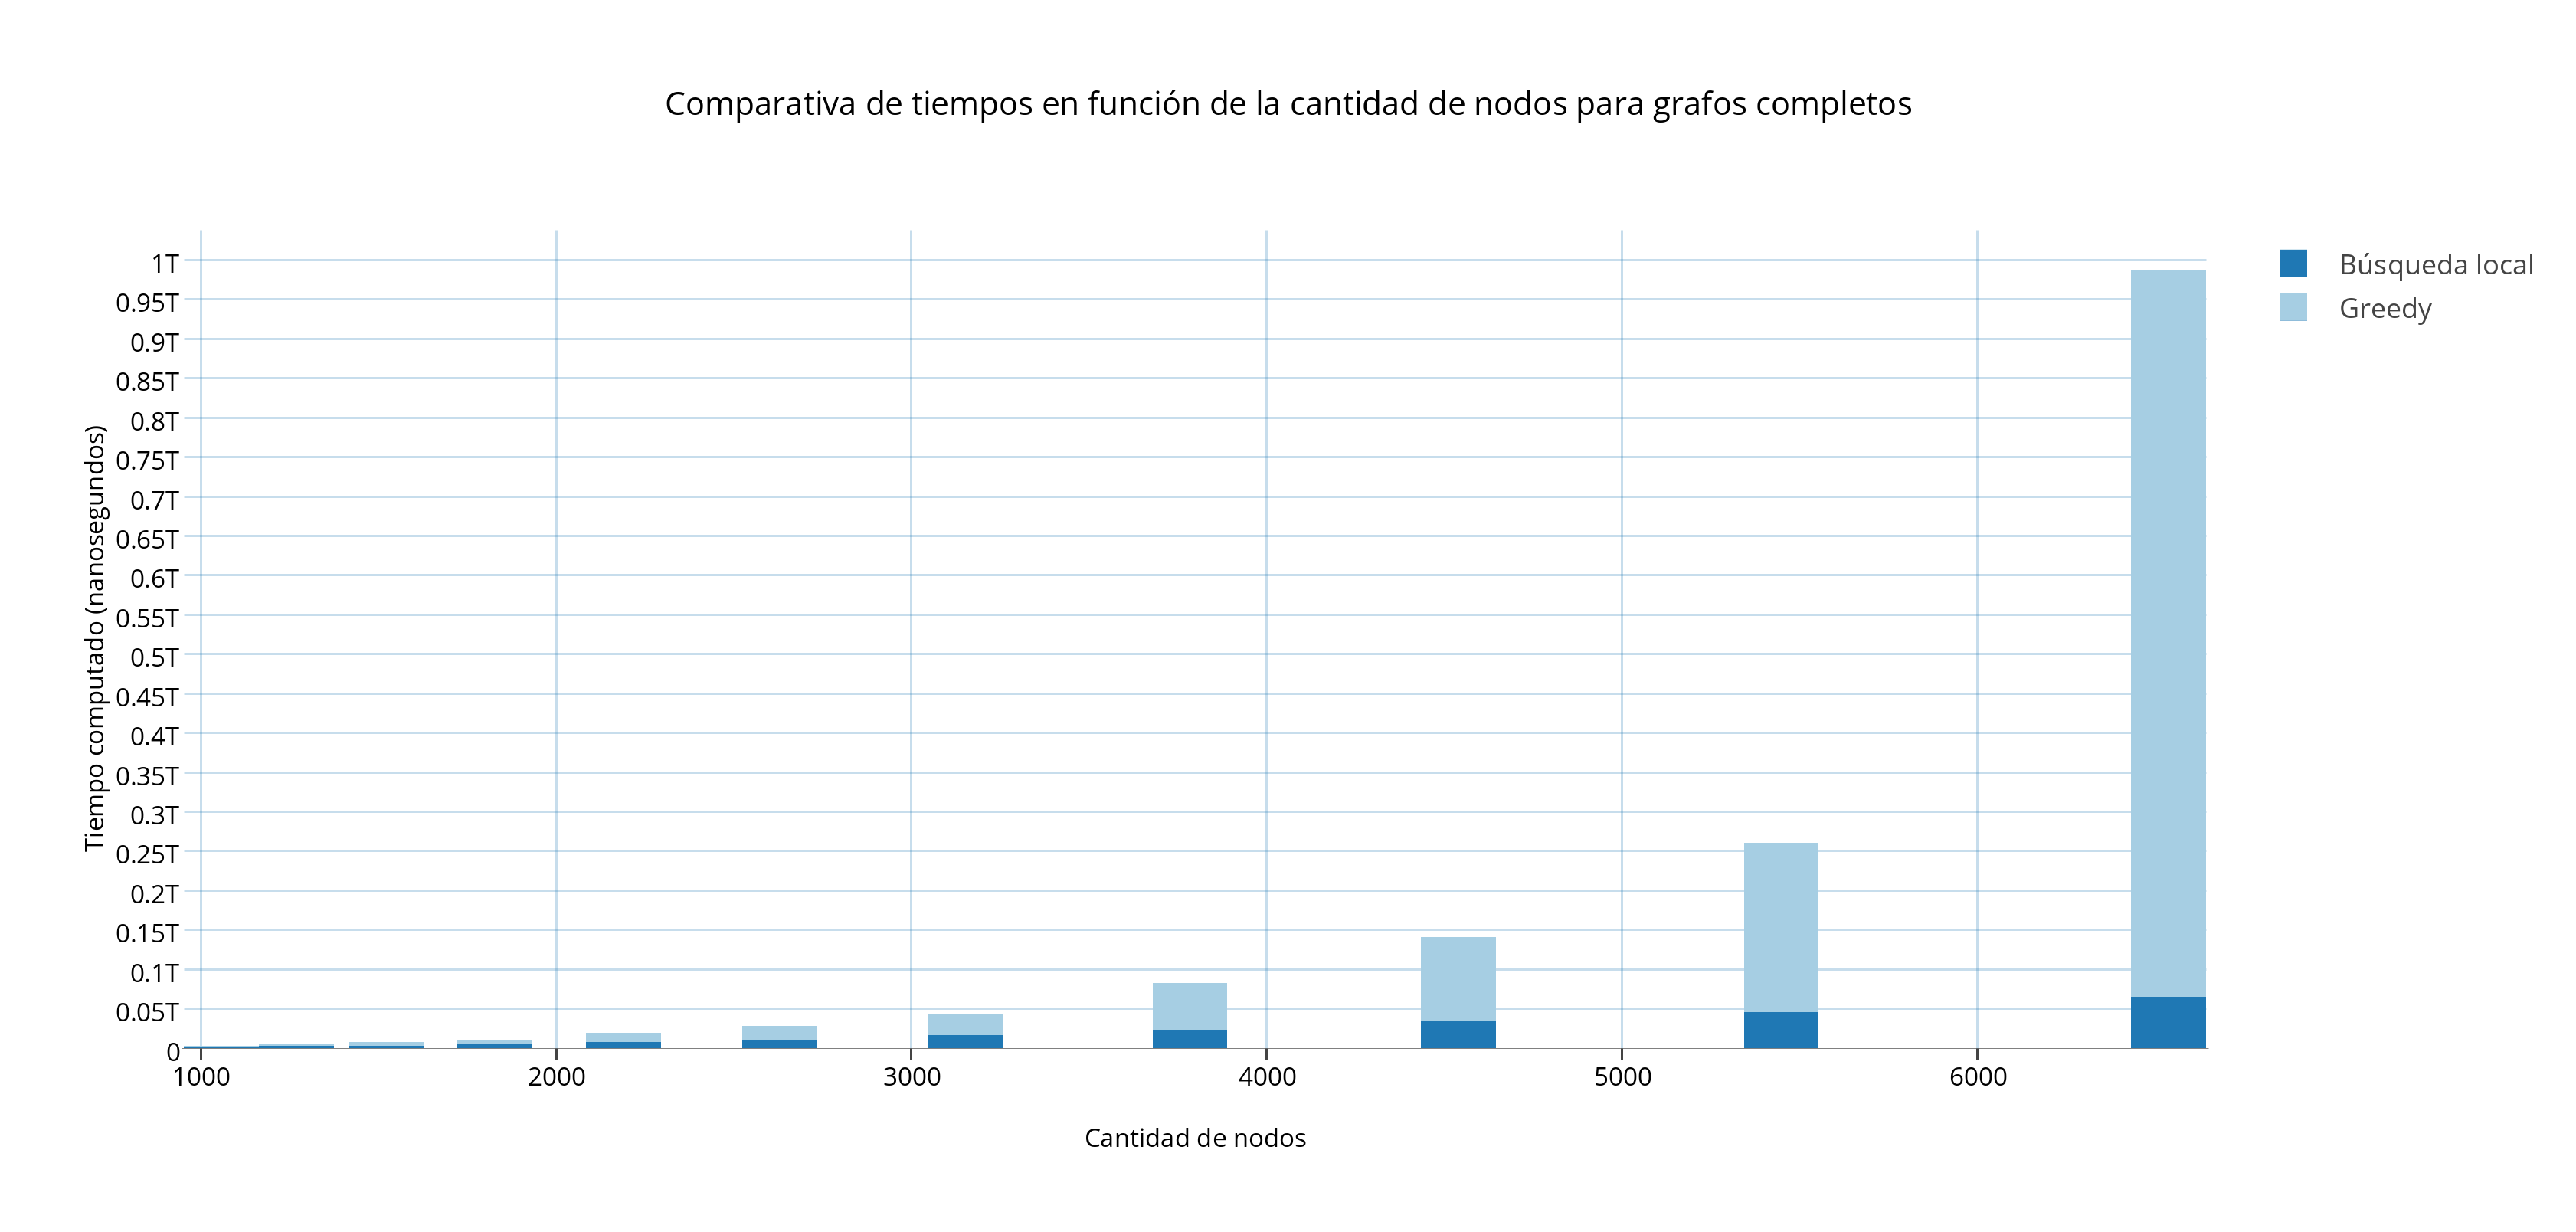
\includegraphics[width=18cm]{imagenes/Ej5/ComparacionTiemposCompleto.png}
 	\label{ComparacionTiemposCompleto}
    \end{center}
  \end{figure}

 \begin{figure}[H]
    \begin{center}
  	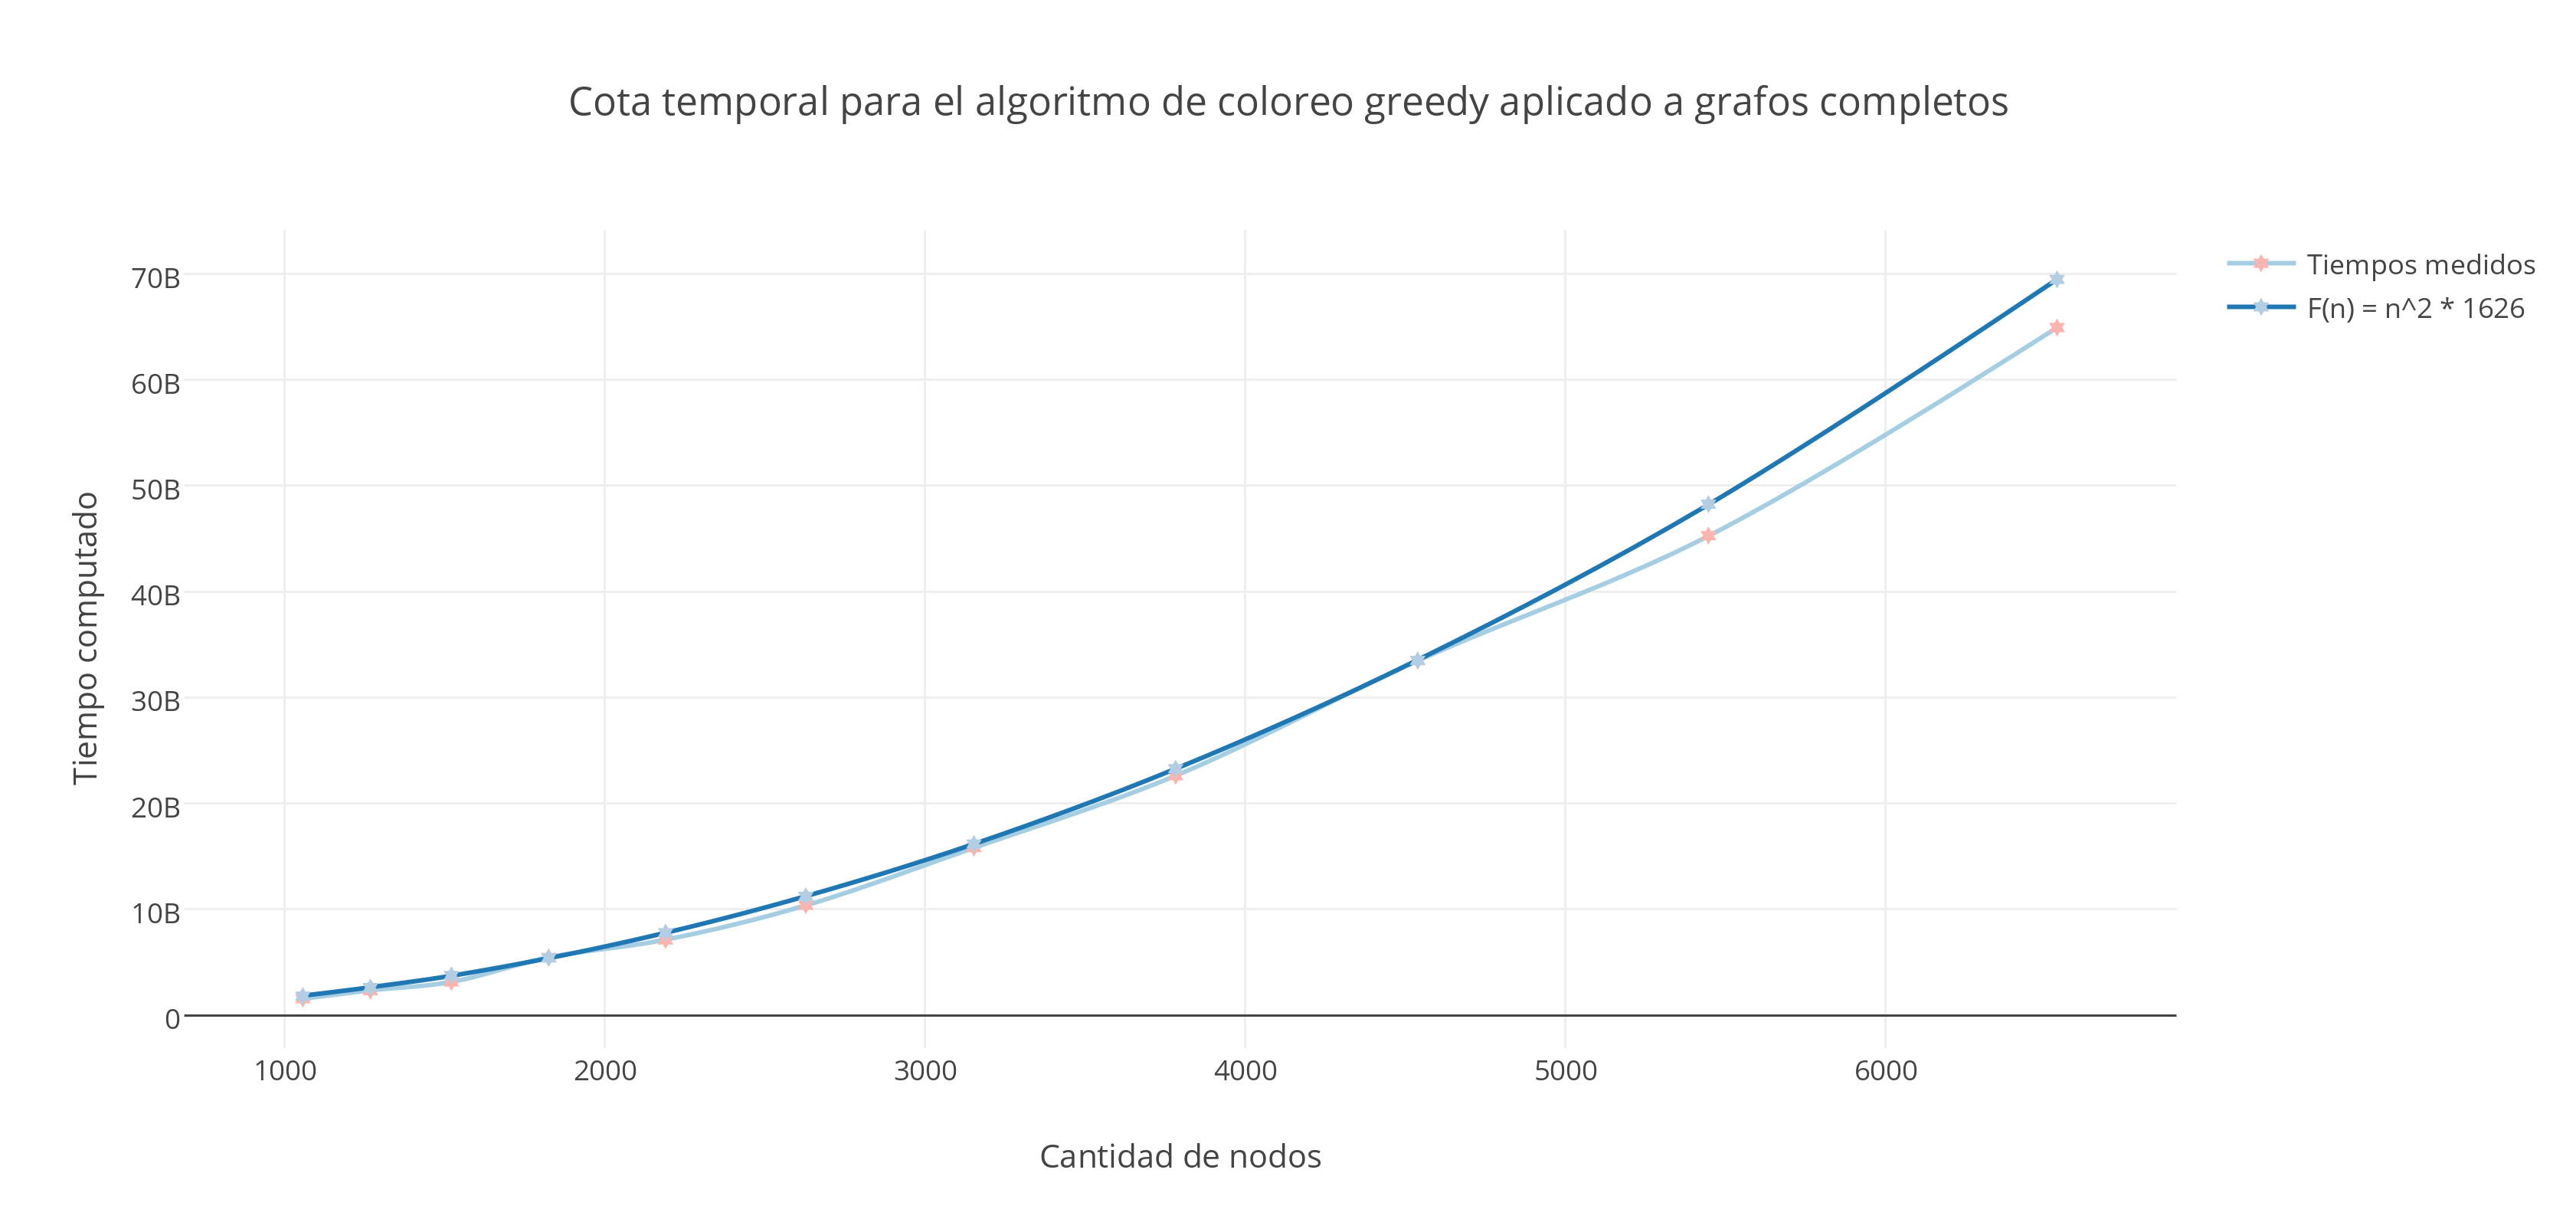
\includegraphics[width=18cm]{imagenes/Ej5/TiempoGreedyCompleto.png}
 	\label{TiempoGreedyCompleto}
    \end{center}
  \end{figure}

 \begin{figure}[H]
    \begin{center}
  	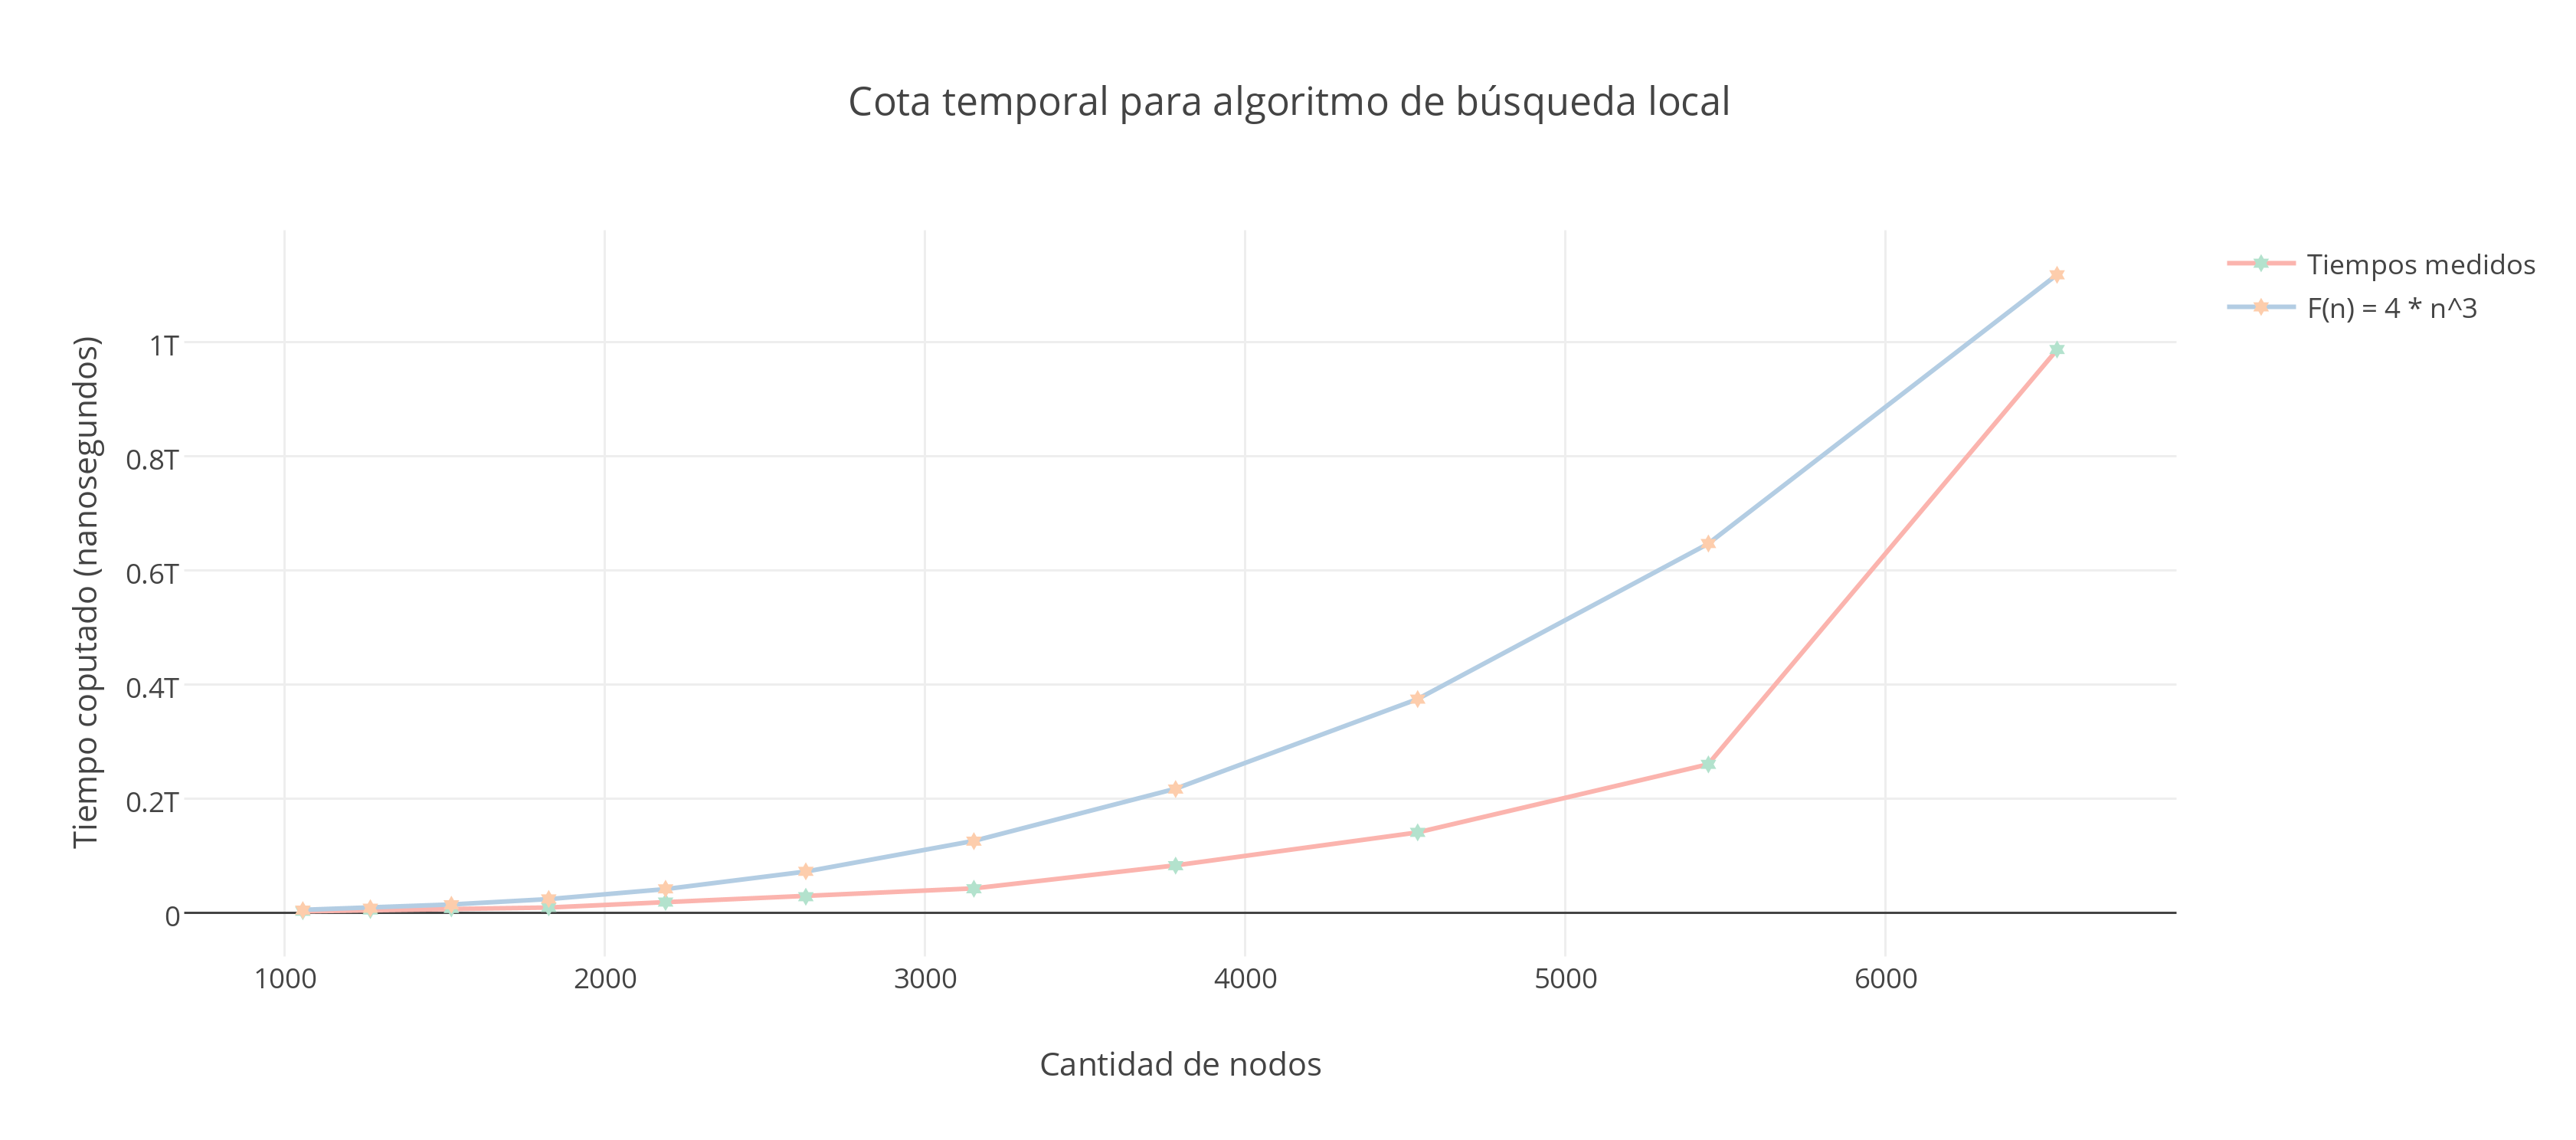
\includegraphics[width=18cm]{imagenes/Ej5/TiemposLocalCompleto.png}
 	\label{TiemposLocalCompleto}
    \end{center}
  \end{figure}

\subsection {Resultados obtenidos a parir de grafos bipartitos completos} 